% Section 1.5: derive arrays from indexed computations before counting costs.
\section{Matrix Dimensions}
\label{sec:logreg_to_mlp:matrix_dimensions}

\subsection{A matrix is an organized collection of scalar equations}
Dimension checking is a way to keep track of meaning: which index identifies an example, which identifies a feature, and which identifies an output neuron? Rather than remembering a transpose by appearance, derive the expression from one output coordinate.

Let $d$ be the input width and $q$ the number of neurons. In the lecture convention, neuron $j$ has a column weight vector $\mathbf{w}_j\in\mathbb{R}^{d\times1}$. Its score is
\[
 z_j=\mathbf{w}_j^{\mathsf T}\mathbf{x}+b_j
     =\sum_{i=1}^d w_{ij}x_i+b_j.
\]
Here $i$ is summed out: it indexes the features contributing to one neuron. The index $j$ survives: it identifies the resulting score. To compute all scores, collect weight vectors into columns,
\[
 W_s=[\mathbf{w}_1\ \cdots\ \mathbf{w}_q]\in\mathbb{R}^{d\times q}.
\]
Then
\[
 \underbrace{\mathbf{z}}_{q\times1}
 =\underbrace{W_s^{\mathsf T}}_{q\times d}
  \underbrace{\mathbf{x}}_{d\times1}
  +\underbrace{\mathbf{b}}_{q\times1},\qquad
 \underbrace{\mathbf{h}}_{q\times1}=g(\underbrace{\mathbf{z}}_{q\times1}).
\]
The subscript $s$ marks the slides' weight storage, to keep it distinct from code notation below. Matrix multiplication performs all the dot products at once; it does not define a different operation from the scalar equations.

\subsection{Batching in the column-vector convention}
Place $B$ examples in columns:
\[
 X_c=[\mathbf{x}^{(1)}\ \cdots\ \mathbf{x}^{(B)}]
 \in\mathbb{R}^{d\times B}.
\]
The batch preactivation matrix has one neuron per row and one example per column:
\begin{equation}
 \underbrace{Z_c}_{q\times B}
 =\underbrace{W_s^{\mathsf T}}_{q\times d}
  \underbrace{X_c}_{d\times B}
  +\underbrace{\mathbf{b}\mathbf{1}_B^{\mathsf T}}_{q\times B},
 \qquad H_c=g(Z_c)\in\mathbb{R}^{q\times B}.
\end{equation}
Entry $(j,n)$ is
\[
 (Z_c)_{jn}=\sum_i(W_s)_{ij}(X_c)_{in}+b_j.
\]
The same $b_j$ is added for every example $n$. Formally, a $q\times1$ matrix cannot be added to a $q\times B$ matrix by ordinary matrix addition. The slides' shorthand ``$+\mathbf{b}$'' means broadcasting, made explicit here by $\mathbf{b}\mathbf{1}_B^{\mathsf T}$. The repeated columns are not different trainable biases.

\subsection{Transpose the whole equation to get row batches}
Code often places examples in rows. Define
\[
 X_r=X_c^{\mathsf T}\in\mathbb{R}^{B\times d},\qquad
 Z_r=Z_c^{\mathsf T}\in\mathbb{R}^{B\times q}.
\]
Using $(AB)^{\mathsf T}=B^{\mathsf T}A^{\mathsf T}$ gives
\begin{align}
 Z_r
 &=\left(W_s^{\mathsf T}X_c+\mathbf{b}\mathbf{1}_B^{\mathsf T}\right)^{\mathsf T}\\
 &=X_c^{\mathsf T}W_s+\mathbf{1}_B\mathbf{b}^{\mathsf T}\\
 &=X_rW_s+\mathbf{1}_B\mathbf{b}^{\mathsf T}.
\end{align}
Since an elementwise activation commutes with transposition,
$H_r=g(Z_r)=H_c^{\mathsf T}$. Nothing about the model has changed.

PyTorch's dense-layer parameter storage uses one neuron's weights per row. Write that matrix as
\[
 W_p=W_s^{\mathsf T}\in\mathbb{R}^{q\times d}.
\]
Consequently, the familiar code expression is
\begin{equation}
 \boxed{\underbrace{Z_r}_{B\times q}
 =\underbrace{X_r}_{B\times d}
  \underbrace{W_p^{\mathsf T}}_{d\times q}
  +\underbrace{\mathbf{1}_B\mathbf{b}^{\mathsf T}}_{B\times q}.}
\end{equation}
This is the formula $Z=XW^{\mathsf T}+B_{\mathrm{bias}}$ in the lecture's coding notation. We use $B_{\mathrm{bias}}$ for the expanded bias matrix so that $B$ alone can denote batch size.

\begin{center}
\begin{tabular}{lll}
\toprule
Object & Lecture columns & PyTorch-style rows\\
\midrule
Batch input & $X_c:d\times B$ & $X_r:B\times d$\\
Stored weights & $W_s:d\times q$ & $W_p:q\times d$\\
Bias as a mathematical column & $\mathbf{b}:q\times1$ & $\mathbf{b}:q\times1$\\
Preactivations & $Z_c:q\times B$ & $Z_r:B\times q$\\
Affine computation & $W_s^{\mathsf T}X_c+\mathbf{b}\mathbf1_B^{\mathsf T}$ & $X_rW_p^{\mathsf T}+\mathbf1_B\mathbf{b}^{\mathsf T}$\\
\bottomrule
\end{tabular}
\end{center}
In NumPy and PyTorch, the bias is typically a one-dimensional array of shape \texttt{(q,)}. It broadcasts over batch rows. A one-dimensional array has no separate row or column orientation; explicitly reshape it when doing column-batch arithmetic.

\begin{warning}[Two independent layout choices]
Changing examples from columns to rows does not logically force a particular weight layout. One could use row batches with $W_s\in\mathbb{R}^{d\times q}$ and write $X_rW_s$, or with $W_p\in\mathbb{R}^{q\times d}$ and write $X_rW_p^{\mathsf T}$. Both are correct. The letters alone do not specify the convention: the index meanings and dimensions do. PyTorch is not a different mathematics.
\end{warning}
The official \href{https://docs.pytorch.org/docs/stable/generated/torch.nn.Linear.html}{\texttt{torch.nn.Linear} documentation} stores weights with output features in rows and input features in columns, using transformation $xA^{\mathsf T}+b$. It also permits leading dimensions beyond a single batch dimension: the last dimension is the feature dimension. Thus ``PyTorch inputs are row vectors'' is a useful two-dimensional batch convention, not a restriction on every supported tensor.

\subsection{Work through every entry of a concrete batch}
Take two examples, three input features, and two neurons:
\[
 X_r=\begin{bmatrix}1&2&3\\-1&0&2\end{bmatrix},\quad
 W_p=\begin{bmatrix}1&-1&2\\0&3&-1\end{bmatrix},\quad
 \mathbf{b}=\begin{bmatrix}0.5\\-0.5\end{bmatrix}.
\]
The product and broadcast bias are
\[
 X_rW_p^{\mathsf T}=\begin{bmatrix}5&3\\3&-2\end{bmatrix},\qquad
 \mathbf1_2\mathbf{b}^{\mathsf T}=\begin{bmatrix}0.5&-0.5\\0.5&-0.5\end{bmatrix}.
\]
For example, the first example's second neuron gives
$1(0)+2(3)+3(-1)-0.5=2.5$. Every other cell follows the same rule:
\[
 Z_r=\begin{bmatrix}5.5&2.5\\3.5&-2.5\end{bmatrix},\qquad
 H_r=\operatorname{ReLU}(Z_r)=\begin{bmatrix}5.5&2.5\\3.5&0\end{bmatrix}.
\]
Row 2 always belongs to example 2; column 2 always belongs to neuron 2. This semantic identity is as important as whether an array multiplication happens to run.

\begin{figure}[htbp]
\centering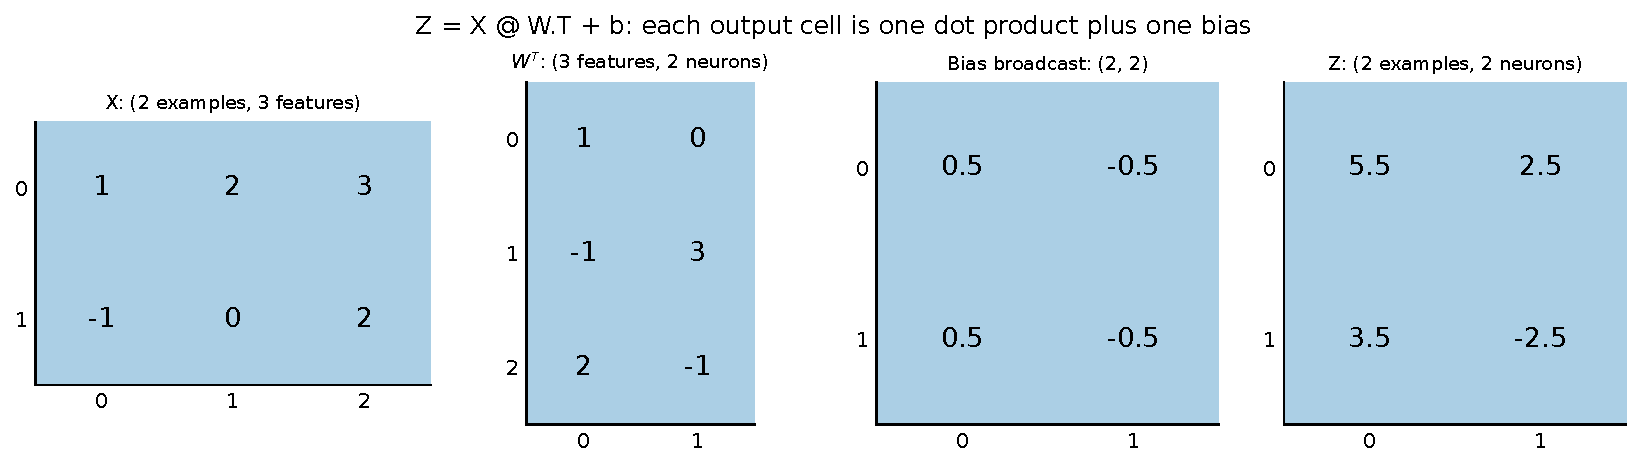
\includegraphics[width=\linewidth]{mlp_1_4_1_5/matrix_example.pdf}
\caption{The batch computation with actual numbers. Output entry $(n,j)$ combines row $n$ of $X$ with column $j$ of $W^{\mathsf T}$, then adds bias $b_j$.}
\end{figure}

\subsection{The lecture's batched-perceptron repetition question}
For one sigmoid output neuron and $B$ examples of dimension $d$, the two requested formulas in row-batch notation are
\begin{align}
 \underbrace{Z}_{B\times1}
 &=\underbrace{X}_{B\times d}
   \underbrace{W^{\mathsf T}}_{d\times1}
   +\underbrace{\mathbf1_B}_{B\times1}\underbrace{b}_{\text{scalar}},
 \qquad W\in\mathbb{R}^{1\times d},\\
 \underbrace{H}_{B\times1}&=\sigma(\underbrace{Z}_{B\times1}).
\end{align}
Equivalently, with examples in columns,
\[
 \underbrace{Z_c}_{1\times B}
 =\underbrace{\mathbf{w}^{\mathsf T}}_{1\times d}
  \underbrace{X_c}_{d\times B}+\underbrace{b\mathbf1_B^{\mathsf T}}_{1\times B},
 \qquad H_c=\sigma(Z_c)\in\mathbb{R}^{1\times B}.
\]
The $B$ probabilities are predictions for different examples, not probabilities of $B$ mutually exclusive classes; there is no reason for them to sum to one.

\subsection{General layer notation and a dimension-checking procedure}
Let there be $L$ computed layers with widths $n_1,\ldots,n_L$, and set $n_0=d$. In row-batch notation,
\[
 H^{(0)}=X\in\mathbb{R}^{B\times d},\qquad
 W^{(\ell)}\in\mathbb{R}^{n_\ell\times n_{\ell-1}},\qquad
 \mathbf{b}^{(\ell)}\in\mathbb{R}^{n_\ell}.
\]
For $\ell=1,\ldots,L$,
\begin{align}
 \underbrace{Z^{(\ell)}}_{B\times n_\ell}
 &=\underbrace{H^{(\ell-1)}}_{B\times n_{\ell-1}}
 \underbrace{W^{(\ell)\mathsf T}}_{n_{\ell-1}\times n_\ell}
 +\underbrace{\mathbf1_B\mathbf{b}^{(\ell)\mathsf T}}_{B\times n_\ell},\\
 \underbrace{H^{(\ell)}}_{B\times n_\ell}&=g^{(\ell)}(Z^{(\ell)}).
\end{align}
To reconstruct this without memory: first decide what an output entry means, $(n,j)$. Then write its feature sum
$Z^{(\ell)}_{nj}=\sum_iH^{(\ell-1)}_{ni}W^{(\ell)}_{ji}+b^{(\ell)}_j$.
The shared feature index $i$ must be contracted; the example and neuron indices survive. This forces the product and its dimensions.

A useful invariant is that the batch dimension stays $B$ through an ordinary MLP. It is the feature width that changes. A square matrix can hide an incorrect transpose; use nonsquare test cases and check values, not shapes alone.

\subsection{General time complexity, then the equal-width answer}
For a batch, layer $\ell$ multiplies $(B\times n_{\ell-1})(n_{\ell-1}\times n_\ell)$. The ordinary algorithm computes $Bn_\ell$ outputs, each using $n_{\ell-1}$ products, so its work is $O(Bn_{\ell-1}n_\ell)$. Bias addition and an elementwise activation each cost $O(Bn_\ell)$. Summing across layers gives
\[
 T=O\!\left(B\sum_{\ell=1}^L n_{\ell-1}n_\ell
             +B\sum_{\ell=1}^L n_\ell\right)
  =O\!\left(B\sum_{\ell=1}^L n_{\ell-1}n_\ell\right).
\]
The simplification assumes positive widths and ordinary coordinatewise activations (or linear-cost softmax). It does not cover arbitrary operations such as self-attention.

For the lecture question, define $M$ to be the number of \emph{computed layers}, all of width $k$, including the output and excluding the input. Then $n_0=d$ and $n_1=\cdots=n_M=k$. The first layer costs $O(Bdk)$ and there are $M-1$ subsequent $k$-to-$k$ maps:
\[
 \boxed{T=O\bigl(Bdk+B(M-1)k^2\bigr).}
\]
For $M\geq2$ it is common to write $O(Bdk+BMk^2)$. Keeping $M-1$ makes the $M=1$ case transparent: it is one layer, so the time is $O(Bdk)$, with no hidden $k^2$ product.

\begin{keyidea}[If ``M layers'' means M hidden layers instead]
State the convention. With $M\geq1$ hidden layers of width $k$ and an additional output of width $c$,
\[
 T=O\bigl(B[dk+(M-1)k^2+kc]\bigr).
\]
For binary classification $c=1$, the last term is $Bk$. For $c=k$, there are $M$ width-$k$ transitions after the input map. Neither output width nor whether it is counted should be silently assumed.
\end{keyidea}

\subsection{General memory complexity: parameters, data, and lifetimes}
Assume parameters for every layer are stored in memory. Count scalar elements; multiply by bytes per element for a storage estimate. The parameter count is
\[
 P=\sum_{\ell=1}^L\bigl(n_{\ell-1}n_\ell+n_\ell\bigr).
\]
It has no factor of $B$: all examples share the same weights and biases. The input takes $Bd$ elements. The final output takes $Bn_L$ elements. The storage of intermediate activations depends on their lifetimes.

\paragraph{Case A: retain the layer activations.}
A simple forward cache stores $Z^{(\ell)}$ and $H^{(\ell)}$ for all layers, for later inspection or differentiation. It requires
\[
 S_{\mathrm{cache}}=P+Bd+2B\sum_{\ell=1}^L n_\ell
 =O\!\left(P+Bd+B\sum_{\ell=1}^L n_\ell\right).
\]
If only one of $Z$ or $H$ is needed, the factor two may disappear. This is still forward-pass storage, not a count of gradients and optimizer buffers.
For $M$ computed layers of width $k$,
\[
 P=dk+(M-1)k^2+Mk,
\]
so the explicit inclusive answer is
\begin{equation}
 \boxed{S_{\mathrm{cache}}
 =O\bigl(dk+(M-1)k^2+Mk+Bd+BMk\bigr).}
\end{equation}
For $B\geq1$, the $Mk$ bias term is bounded by $BMk$, yielding
$O(dk+(M-1)k^2+Bd+BMk)$.
This is the standard answer when ``memory of the forward pass'' includes retaining all layer results. It follows the hint by counting parameters, inputs, and outputs rather than multiplying their sizes.

\paragraph{Case B: forward-only inference with buffer reuse.}
An ordinary sequential MLP only needs the previous activation to compute the next one. Once consumed, earlier buffers can be discarded. A conservative accounting keeps the original input resident, plus current layer input, preactivation, and output. Therefore
\[
 S_{\mathrm{infer}}
 =O\!\left(P+Bd+B\max_{1\leq\ell\leq L}(n_{\ell-1}+n_\ell)\right).
\]
Any double counting of the original input changes only a constant. For equal width,
\begin{equation}
 \boxed{S_{\mathrm{infer}}
 =O\bigl(dk+(M-1)k^2+Mk+Bd+Bk\bigr).}
\end{equation}
The parameters still grow with depth, but the live activation buffers need not. The two answers describe different implementations; a question that does not specify retention is best answered by stating the assumption and giving the distinction.

\begin{figure}[htbp]
\centering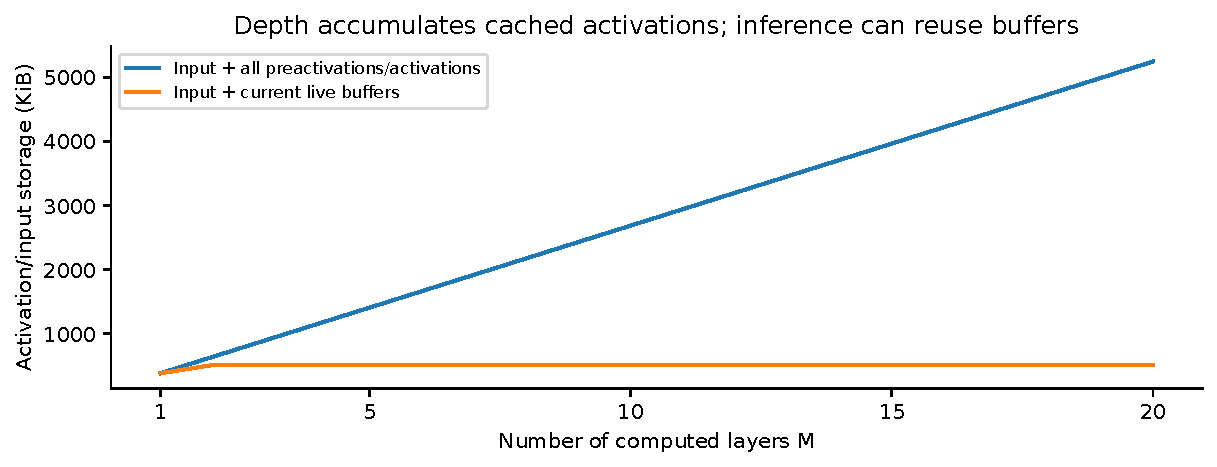
\includegraphics[width=\linewidth]{mlp_1_4_1_5/activation_memory.pdf}
\caption{Storage for input and activations at $B=512$, $d=k=64$. The cached implementation stores both $Z$ and $H$ for every layer. The inference model retains the input and only live layer buffers. Parameters are excluded from this plot to isolate activation lifetime; they must be added for total memory. These are calculated array sizes, not measured runtime allocations.}
\end{figure}

Do not sum each layer's full memory formula mechanically and count the same weights or boundary activation twice as distinct objects. Count distinct stored arrays, then decide which coexist. Likewise, multiplying a $B\times d$ batch by a $d\times k$ matrix does not require a $B\times d\times k$ tensor of all scalar products; standard matrix multiplication accumulates into the $B\times k$ output.

\paragraph{What happens to the expanded bias?}
Mathematically $\mathbf1_B\mathbf{b}^{\mathsf T}$ has $Bk$ entries, but broadcasting need not allocate a separate dense repeated copy. There remain only $k$ learned bias parameters. Explicitly materializing the repeated matrix adds a $Bk$ temporary; the activation order is unchanged, but practical memory use increases.

\begin{figure}[htbp]
\centering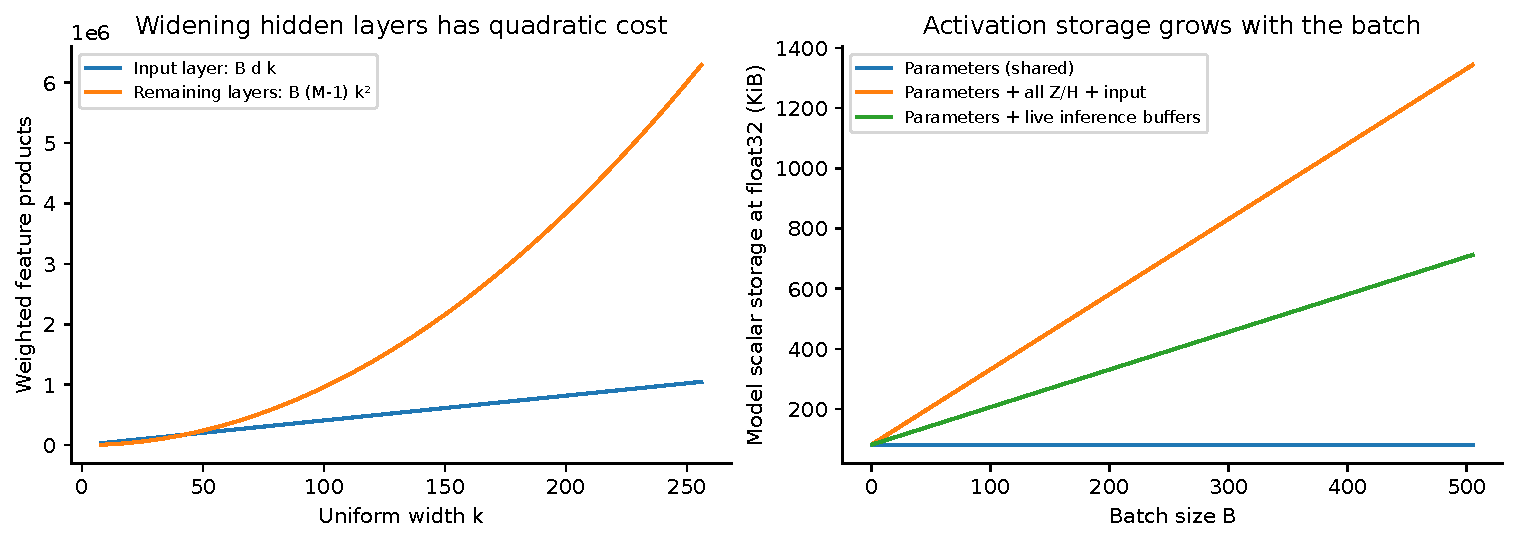
\includegraphics[width=\linewidth]{mlp_1_4_1_5/complexity_scaling.pdf}
\caption{Left: ordinary multiplication counts for four width-$k$ computed layers, $B=32$, $d=128$. Right: a four-layer model with $d=128$, $k=64$ and variable batch size. Weights are reused across examples, while activation/input storage grows with $B$. Curves are analytic counts, not timing measurements.}
\end{figure}

\subsection{A numerical batch budget and what it teaches}
Return to the $12\to32\to16\to1$ grasp model. At $B=256$, the input has 3,072 entries and all $Z/H$ arrays have $2(256)(49)=25,088$ entries. Including 961 parameters yields
\[
 S_{\mathrm{cache}}=29{,}121\text{ scalars}=116{,}484\text{ bytes at float32}.
\]
One conservative inference implementation, keeping the input plus separate live input/$Z$/$H$ buffers, peaks at 16,384 live intermediate scalars, hence
\[
 S_{\mathrm{infer}}=961+3{,}072+16{,}384=20{,}417\text{ scalars}.
\]
The live intermediate maximum is attained by $2B(32)$ in the first layer or $B(32+2\cdot16)$ in the second. In-place activation or fused kernels can reduce this number. These precise counts belong to the stated storage model, whereas the big-O expressions describe scaling robustly across such constant-factor changes.

Larger batches increase arithmetic and activation storage but not parameter count. Wider hidden layers can increase matrix work quadratically because both ends of a dense connection grow. More layers increase weight storage and computation approximately linearly at fixed width; retained activations also accumulate with depth. These observations help reason about embedded inference and GPU batch sizing before running an experiment.

\subsection{NumPy implementation: translate the equations literally}
\begin{lstlisting}
import numpy as np

X = np.array([[1., 2., 3.], [-1., 0., 2.]])  # (B=2, d=3)
W = np.array([[1., -1., 2.], [0., 3., -1.]]) # (q=2, d=3)
b = np.array([0.5, -0.5])                    # (q=2,)
Z = X @ W.T + b                             # (B=2, q=2)
H = np.maximum(Z, 0.0)                      # (B=2, q=2)
np.testing.assert_allclose(Z, [[5.5, 2.5], [3.5, -2.5]])

# The same calculation in the slide convention:
Xc = X.T                                   # (d=3, B=2)
Ws = W.T                                   # (d=3, q=2)
Zc = Ws.T @ Xc + b[:, None]                 # (q=2, B=2)
np.testing.assert_allclose(Z, Zc.T)
\end{lstlisting}
For a network, each layer consumes the previous layer's output:
\begin{lstlisting}
H = X
for ell, (W, b) in enumerate(zip(weights, biases)):
    Z = H @ W.T + b
    if ell < len(weights) - 1:
        H = np.maximum(Z, 0.0)              # hidden ReLU
    else:
        H = np.exp(-np.logaddexp(0.0, -Z)) # stable sigmoid
\end{lstlisting}
This code assumes a binary or independent-sigmoid output, not a mutually exclusive multiclass softmax. No labels are needed to produce predictions. Labels enter when computing a loss.

Beware of \texttt{X * W}: it is elementwise multiplication, not a collection of dot products. Also, \texttt{np.zeros(d).T} still has shape \texttt{(d,)}; transpose does not turn a one-dimensional array into a column. Use \texttt{x[:, None]} for \texttt{(d,1)} or \texttt{x[None, :]} for \texttt{(1,d)}. For loss calculations, keep both targets and predictions consistently \texttt{(B,)} or consistently \texttt{(B,1)}: subtracting arrays of these two different shapes can silently create a \texttt{(B,B)} result.

\subsection{Exercises with worked answers}
\paragraph{1. Recover the matrix dimensions.}
A batch has 8 examples with 6 features and a layer has 5 neurons. In row notation,
$X:8\times6$, $W:5\times6$, $b:5$, $Z,H:8\times5$.
In column notation, $X_c:6\times8$, $W_s:6\times5$, and $Z_c,H_c:5\times8$.
Both compute 240 scalar weight products and use 35 trainable parameters.

\paragraph{2. Check the boundary cases of the complexity answer.}
At $M=1$, $T=O(Bdk)$, and inclusive memory is $O(dk+k+Bd+Bk)$. At $B=1$, the general batch formulas reduce to single-example formulas. If $d=k$ and $M\geq1$, time simplifies to $O(BMk^2)$. Checking these cases can reveal an incorrectly counted input layer or an extra hidden layer.

\paragraph{3. Does doubling batch size double total memory?}
Write $S=P+A(B)$ where $P$ is fixed parameter storage and $A(B)$ is linear in $B$ under a fixed buffering policy. Then $S(2B)=P+2A(B)$, which is generally less than $2S(B)$. It approaches twice as much only when batch-dependent storage dominates.

\paragraph{4. Why not multiply the parameter count by B?}
A parameter defines the same function for every example. Batching evaluates that one function repeatedly. For an ordinary MLP, permuting the batch rows permutes output rows in exactly the same way; it does not change the parameters or mix information between examples.

\paragraph{5. Why can a shape-correct expression still be wrong?}
If $B=d=q$, several incorrect transposes and bias placements produce compatible square shapes. They can combine examples instead of features or associate biases with examples. Evaluate a small nonsquare example against scalar loops to test the intended index semantics. The companion script checks this equivalence, verifies row/column conversion, and compares batched predictions with one-example-at-a-time predictions.

\paragraph{Reproducible companion.}
Run \texttt{python deep\_learning/code/mlp\_1\_4\_1\_5.py} from the repository root. It verifies the numerical examples and parameter/cache counts, demonstrates affine collapse and XOR, and regenerates all four figures. Its memory plots count array elements under explicit buffering assumptions and do not claim measured CPU/GPU memory or latency.
